\documentclass[main]{subfiles}


\begin{document}
\newpage
\section{Plasticity In The Brain}

%---------------------------
\subsection{Why do we need plasticity?}
Why this topic is relevant:
\begin{itemize}
    \item Biological plasticity might provide a different angle to understand the training procedures in DNNs.
    \item Given the effectiveness of human brain learning bio-plasticity might provide inspiration/new ideas for improved DNN training algorithms.
    \item Understanding biological plasticity might help to better understand how (hierarchical) learning is organized in the brain (Learning and Memory).
    \item Many neural disorders such as dementia might relate to a disturbance in neuronal plasticity that cause neuronal networks to become dysfunctional. Some plasticity mechanisms /disorders lead to malfunction in the brain.
\end{itemize}

\textbf{Plasticity}: allows acquisition of knowledge/information and the formation of memory through experience

\textbf{Memory}: as storage of information that can be recalled later

\textbf{Note}: learning results in memory - which has further outcome - it can change future behavior

\begin{figure}[H]
    \centering
    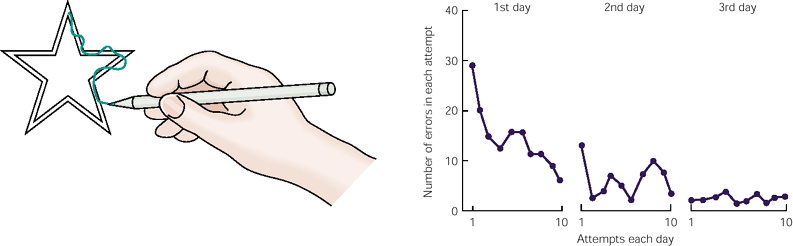
\includegraphics[width=\textwidth]{03_PlasticityInTheBrain/figures/motorlearning.jpg}
    \caption{Motor learning task. Some human subjects have got the task to draw. Having gotten an (electrical) feedback, this subjects learned the pattern they had to draw\footnote{Kandel, \textit{Principles of neural science}, 2001}, according to the motto: ``Here I get a reward, here not\ldots''}
    \label{fig:motorlearning}
\end{figure}

However, everything we do is \textit{learning} and for that we need \textit{plasticity}.

%---------------------------
\subsection{Synaptic Plasticity}

\subsubsection{Biological Recap}
In synaptic plasticity one understands changes in reactivity of \textbf{post}- to \textbf{pre}synaptic neuron. In other words, plasticity changes of chemical synapses can strengthen or weaken transmission. This changes can last from milliseconds (short-term) to weeks or longer (long-term).

Some definitions:
\begin{itemize}
    \item \textbf{EPSP}: Excitatory postsynaptic potential
    \item \textbf{LTP}: long term potentiation; long lasting increase in synaptic strength, i.e. EPSP amplitude
    \item \textbf{LTD}: long term depression; long lasting decreaes in synaptic strenth
\end{itemize}

\textbf{Recap of Synaptic Plasticity} (\textit{see} Figure \ref{fig:syn_plast}):
\begin{enumerate}
    \item AP comes in,
    \item \ce{Ca^2+} channels open, \ce{Ca^2+} influx and causes
    \item neurotransmitter (NT) release.
    \item NT cross synaptic cleft and
    \item bind to postsynaptic receptors, e.g. AMPA receptor to increase probability of depolarisation
\end{enumerate}

\begin{figure}[H]
    \centering
    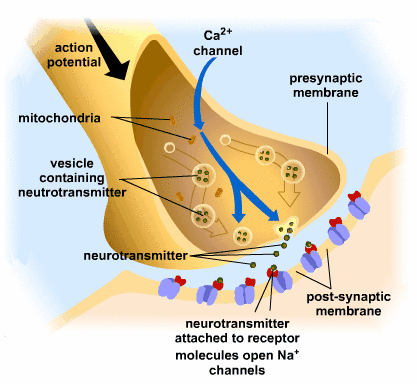
\includegraphics[width=.7\textwidth]{03_PlasticityInTheBrain/figures/synaptic_plasticity.jpg}
    \caption{Short recap of synaptic plasticity.}
    \label{fig:syn_plast}
\end{figure}

\textbf{QUIZ}:
\begin{itemize}
    \item What are the differences between the weights of a deep network and the connections between biological neurons?
    \item Is synaptic plasticity the only mechanism that neurons can use to alter their effective connectivity?
    \item Is weight tuning by BP the only mechanism in DNNs that affect the weights?
\end{itemize}

\subsubsection{Homeostatic Plasticity}
\subsubsection{Hebb’s Idea and STDP}
\subsubsection{Heterostatic Plasticity}
\subsubsection{Behavior time scale Plasticity}
\subsubsection{Time scales of synaptic plasticity (short term, LTP/LTD)}

%---------------------------
\subsection{The Hippocampus as a model system to study neural plasticity}
\subsubsection{LTP and LTD induction in the Hippocampus}
\subsubsection{Molecular basis of synaptic plasticity}

%---------------------------
\subsection{Non-synaptic plasticity}
\subsubsection{Neuronal excitability and spike generation}
\subsubsection{Axonal modulation (shunting, frequency filtering)}
\subsubsection{Alterations of dendritic excitability}


\end{document}